\documentclass[twocolumn, 11pt]{article}

\usepackage[brazilian]{babel}
\usepackage[utf8]{inputenc}
\usepackage{indentfirst}

\usepackage[utf8]{inputenc}
\usepackage{mathtools}
\usepackage{color}
\usepackage{geometry}
\usepackage{listings}

% Tamanho das margens:
\geometry{
	a4paper,
	total={170mm,257mm},
	left=20mm,
	top=20mm,
}

% Definir cores personalizadas
\definecolor{codegreen}{rgb}{0,0.6,0}
\definecolor{codegray}{rgb}{0.5,0.5,0.5}
\definecolor{codepurple}{rgb}{0.58,0,0.82}
\definecolor{backcolour}{rgb}{0.961, 0.961, 0.961}
\definecolor{keywordcolour}{rgb}{0.8,0,0.4}
\definecolor{labelcolour}{rgb}{0.31, 0.4, 0.741}

% Configurar linguagem Assembly personalizada
\lstdefinelanguage{Assembly}{
    morekeywords={brzr, ji, ld, st, addi, jr, addiu, inc, not, and, or, xor, add, sub, slr, srr},
    keywordstyle=\color{keywordcolour}\bfseries,
    morekeywords=[2]{main:, loop_AB:, loop_R:}, 
    keywordstyle=[2]\color{labelcolour}\bfseries, 
    comment=[l]{;},
    commentstyle=\color{codegreen}\itshape,
    morestring=[b]",
    stringstyle=\color{codepurple},
    sensitive=true,
    alsoletter=:
}

\lstdefinestyle{mystyle}{
    backgroundcolor=\color{backcolour},   
    basicstyle=\fontsize{7}{8}\selectfont\ttfamily,
    breakatwhitespace=false,         
    showspaces=false,                
    tabsize=1,
    language=Assembly
}

\lstset{style=mystyle}

\author{Andrieli Luci Gonçalves}
\title{Relatório do Trabalho 2 de Arquitetura de Computadores - CI1212}

\begin{document}

\maketitle        

\section{Introdução}

Este relatório descreve a implementação de um processador monociclo, baseado na arquitetura 8-bits REDUX-V, bem como o desenvolvimento de um programa em Assembly que realiza a soma de dois vetores (A e B) e armazena em um vetor R.

O trabalho foi realizado a partir das seguintes etapas: criação de diagramas do projeto do caminho de dados e da Unidade Lógica e Aritmética (ULA), implementação do processador monociclo no software \textit{Logisim Evolution 3.9.0}, reescrita do Trabalho 1 com a inclusão de três novas instruções Assembly e adaptação do processador para contemplar essas novas instruções. 

\section{Projeto}

\subsection{Processador}

O projeto do processador é composto pelos seguintes componentes: \textit{Program Counter (PC)}, Memória de Instruções e Dados (RAM), Memória de Controle (ROM), Banco de Registradores, ULA e auxiliares — como multiplexadores, somadores e extensores de sinal/zero.

Ademais, para que o Banco de Registradores e o PC realizassem uma comunicação coerente com a Memória de Instruções e Dados, os dois primeiros deveriam ter duração de \textit{2 ticks} com \textit{offset} de \textit{1 tick}, ao passo que a memória, \textit{1 tick} para duração e offset.

\begin{figure}[h]
    \centering
    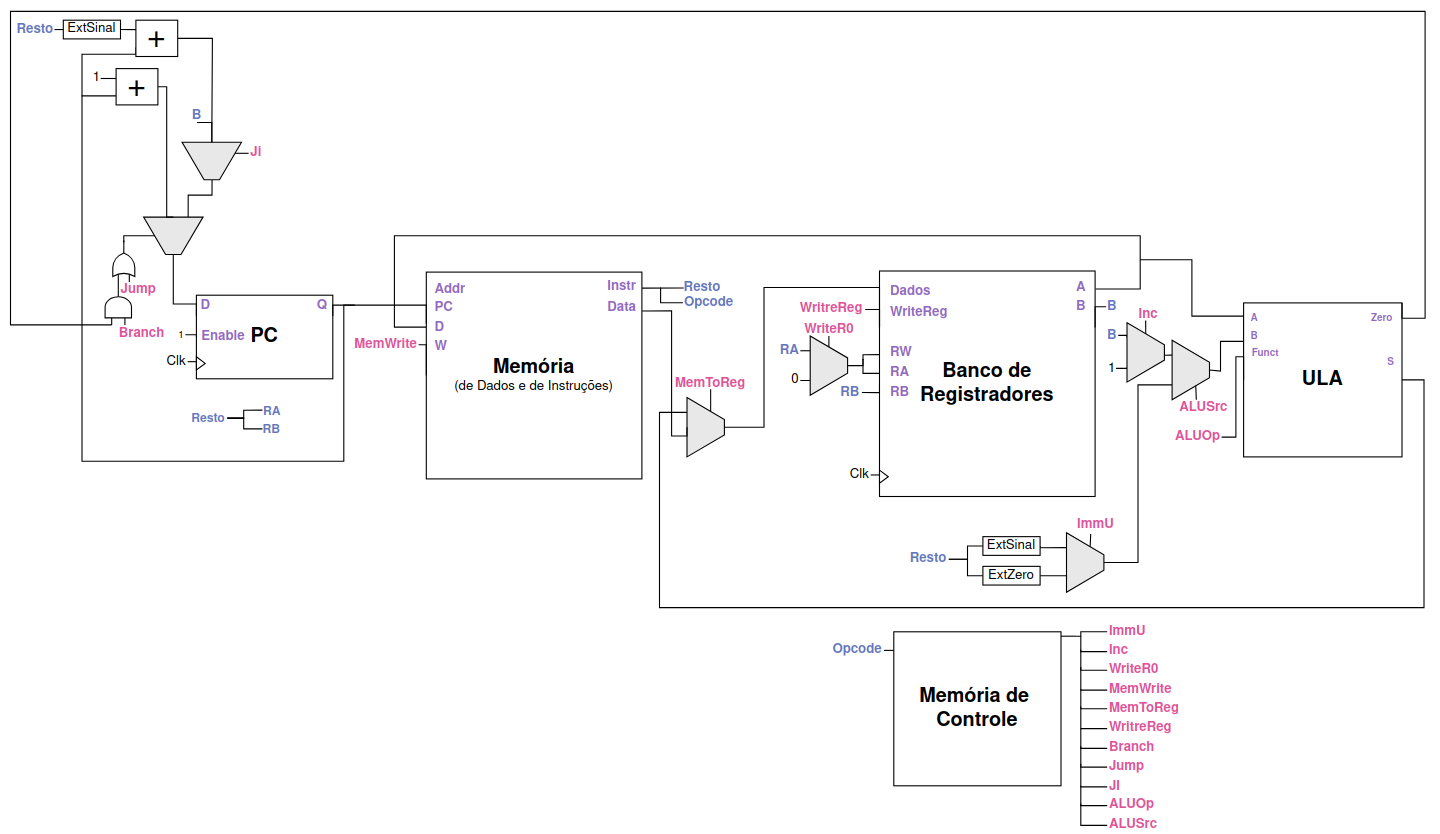
\includegraphics[width=0.9\linewidth]{datapath_processador.png}
    \caption{Diagrama de caixas do caminho de dados do processador.}
    \label{fig:enter-label}
\end{figure}

\subsubsection{Memória de controle}

Para a execução das instruções, foram definidos os seguintes sinais de controle:

\begin{itemize}
    \item \texttt{ImmU}: identifica se para o imediato é necessário considerar o seu sinal. Se sim, ele é extendido, caso contrário a extensão é com zero;
    \item \texttt{Inc}: ativo quando a instrução é a de incremento;
    \item \texttt{WriteR0}: habilita exclusivamente a leitura e escrita no registrador \texttt{R0};
    \item \texttt{MemWrite}: habilita escrita na memória;
    \item \texttt{MemToReg}: habilita escrita no registrador a partir de um dado da memória;
    \item \texttt{WriteReg}: habilita escrita no registrador; 
    \item \texttt{Branch}: indica se a instrução processada é um salto condicional;
    \item \texttt{Jump}: indica se a instrução processada é um salto incondicional;
    \item \texttt{JI}: indica se o salto incondicional depende de um valor imediato;
    \item \texttt{ALUOp}: operação a ser realizada pela ULA; 
    \item \texttt{ALUSrc}: ULA deve receber um operando imediato ou proveniente de um registrador.
\end{itemize}

\subsection{ULA}

Suas operações foram codificadas considerando os três bits menos significativos das instruções lógico-aritméticas da arquitetura, indo, portanto, de \texttt{000} (0) até \texttt{111} (7). Além da saída referente ao resultado da operação, há também o \texttt{Zero}, cujo propósito é indicar se o operando \texttt{A} é igual a zero.

Para todas as operações, foram utilizados os componentes prontos do simulador.

A seguir, tem-se o diagrama do projeto interno da ULA:

\begin{figure}[h]
    \centering
    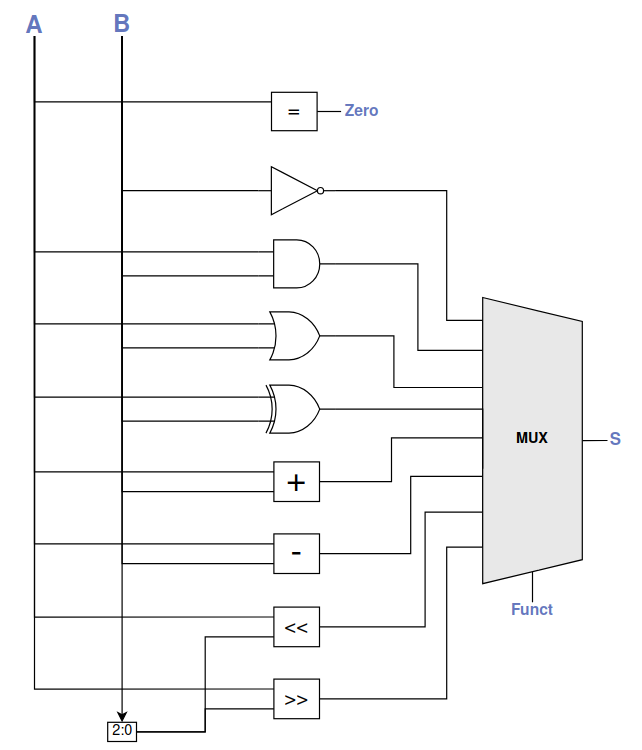
\includegraphics[width=0.9\linewidth]{projeto_ula.png}
    \caption{Diagrama de caixas da ULA.}
    \label{fig:enter-label}
\end{figure}

\section{Programa}

De forma resumida, a sequência lógica utilizada para resolver o problema da soma dos vetores foi, a princípio, guardar em endereços específicos da memória o valor de salto da instrução \texttt{brzr}, tal qual o tamanho dos vetores. Em endereços seguintes, seriam guardados os valores dos vetores \texttt{A}, \texttt{B} e \texttt{R}. Os vetores \texttt{A} e \texttt{B} eram preenchidos simultaneamente, de modo que o laço de repetição ia de um para o outro adicionando os novos valores. O resultado da soma seguia a mesma proposta.

\subsection{Novas instruções}

A partir do código implementado no Trabalho 1, foram anotadas as seguintes dificuldades: limitação do imediato em instruções do tipo I (visto que ele só poderia ser representado a partir de números com sinal e de 4 bits), necessidade de incrementar valores dos registradores em uma unidade e, por fim, a restrição nos saltos incondicionais —, também associados ao imediato.

Assim, para o Trabalho 2, foram idealizadas as seguintes instruções:

\begin{itemize}
    \item \texttt{inc}: incrementa em 1 o valor armazenado no registrador \texttt{RA};
    \item \texttt{addiu}: seu papel é adicionar ao registrador \texttt{R0} um imediato sem sinal, contemplando os valores de 0 a 15;
    \item \texttt{jr}: salto incondicional com base no valor presente em um registrador.
\end{itemize}

No que tange ao conjunto de instruções da arquitetura REDUX-V, pode-se apresentar as novas do seguinte modo:

\begin{center}
\scriptsize
\renewcommand{\arraystretch}{1.1} % Espaçamento entre linhas
\setlength{\tabcolsep}{2pt} % Espaçamento entre colunas
\begin{tabular}{|c|c|p{2cm}|p{2cm}|}
\hline
\textbf{Mnemônico} & \textbf{Opcode} & \textbf{Nome} & \textbf{Operação} \\ \hline
\texttt{inc} & 0101 & Increment & \texttt{R[ra] = R[ra] + 1} \\ \hline
\texttt{addiu} & 0110 & Add Immediate Unsigned & \texttt{R[0] = R[0] + ImmUnsigned} \\ \hline
\texttt{jr} & 0111 & Jump Register & \texttt{PC = R[rb]} \\ \hline
\end{tabular}
\end{center}

Após integrar as novas instruções ao projeto, houve uma mudança na lógica de execução: agora, o valor de salto do \texttt{jump} também pode ser obtido a partir de um registrador (assim como \texttt{brzr}. Desse modo, não é mais necessário realizar saltos intermediários para alcançar a posição desejada.

\subsection{Código em Assembly}

\begin{lstlisting}
; -- tamanho do vetor --
addiu 10     ; r0 = 10
add r1, r0   ; r1 = 10

; -- definindo num da inst. do jump (loop A/B) --
addiu 9      ; r0 = 19
add r2, r0   ; r2 = 19

; -- definindo num da inst. do branch (loop A/B) --
add r0, r0   ; r0 = 19 + 19 = 38
addi 6       ; r0 = 38 + 6 = 44
add r3, r0   ; r3 = 44

; -- guarda na memoria valor do jump (loop A/B) --
sub r0, r0   ; zera r0
addi 5       ; r0 = 5 
slr r0, r0   ; r0 = (5 * 2^5) = 160
st r2, r0    ; guarda 19 na posicao 160

; -- guarda na memoria valor do branch (loop A/B) --
inc r0       ; incrementa r0
st r3, r0    ; guarda 44 na posicao 161

; -- guardando tamanho do vetor --
inc r0       ; incrementa r0
st r1, r0    ; guarda 10 na posicao 162

; -- posicao inicial do vetor -- 
inc r0       ; incrementa r0
sub r1, r1   ; zera r1
add r1, r0   ; r1 = 163

sub r3, r3   ; zera r3

loop_AB:    sub r0, r0  ; zera r0
            sub r2, r2  ; zera r2
            inc r2      ; incrementa r2

            st r3, r1   ; M[r1] = r3 (A)
            inc r3      ; r3 = r3 + 1
            addiu 10    ; r0 = 10
            add r1, r0  ; avanca r1 em 10 posicoes
            st r3, r1   ; M[r1] = r3 (B)
            sub r1, r0  ; retorna r1 em 10 posicoes

            addi -5     ; r0 = 5
            slr r0, r0  ; r0 = (5 * 2^5) = 160
            addi 2      ; r0 = 162
            ld r3, r0   ; r3 = M[r0]
            sub r3, r2  ; r3 = r3 - 1
            st r3, r0   ; guarda r3-- na posicao 162
            addi -1     ; r0 = 161
            ld r2, r0   ; r2 = M[r0] = 161
            brzr r3, r2 ; r3 = 0, vai p/ inst 44

            addi -1     ; r0 = 160
            ld r2, r0   ; r2 = M[r0]

            ld r3, r1   ; r3 = M[r1]
            inc r1      ; incrementa r1
            inc r3      ; incrementa r3
            inc r3      ; incrementa r3

            jr r2       ; volta p/ inst 19

sub r0, r0   ; zera r0

; -- recalcula num da inst. do jump (loop R) --
addiu 14     ; r0 = 14
add r2, r0   ; r0 = 14 + 44 = 58
add r3, r0   ; r3 = 14
addi -2      ; r0 = 12
sub r1, r0   ; r1 = 160
st r2, r1    ; M[r1] = r2

; -- recalcula num da inst. do branch (loop R) --
inc r1       ; incrementa r1 (161)
add r2, r3   ; r2 = 58 + 14 = 72
add r2, r0   ; r2 = 72 + 12 = 84
st r2, r1    ; M[r1] = r0

; -- recalcula tamanho do vetor (loop R) --
inc r1       ; incrementa r1 (162)
addi -2      ; r0 = 10
st r0, r1    ; M[r1] = 10 (tam vetor)

loop_R:     inc r1       ; incrementa r1
            sub r0, r0   ; zera r0
            ld r3, r1    ; r3 = M[r1]
            addi 5       ; r0 = 5
            addi 5       ; r0 = 10
            add r1, r0   ; vai para vetor B
            ld r2, r1    ; r2 = M[r1]
            add r3, r2   ; r3 = r3 + r2 (R = A + B)
            add r1, r0   ; vai para vetor R
            st r3, r1    ; M[r1] = r3
            sub r1, r0   ; volta para vetor B
            sub r1, r0   ; volta para vetor A

            addi -5      ; r0 = 5
            slr r0, r0   ; r0 = (5 * 2^5) = 160
            addi 2       ; r0 = 162
            ld r3, r0    ; r3 = M[r0]
            sub r2, r2   ; zera r2
            inc r2       ; incrementa r2
            sub r3, r2   ; decrementa r3
            st r3, r0    ; M[r0] = r3
            addi -1      ; r0 = 161
            ld r2, r0    ; r2 = M[r0]
            brzr r3, r2  ; r3 = 0, vai p/ inst 84

            addi -1      ; r0 = 160
            ld r2, r0    ; r2 = M[r0]

            jr r2        ; volta p/ inst 58

ji 0   ; finaliza programa
\end{lstlisting}

\end{document}